\renewcommand{\thechapter}{\Alph{chapter}}
\chapter{Opis techniczny platformy}
\label{cha:opis_techniczny}

\section{Oprogramowanie ArduPilot}
Oprogramowanie ArduPilot jest jednym z najbardziej popularnych systemów instalowanych na kontrolerach lotu. Jest to projekt open source, którego największą zaletą jest bogata możliwość konfiguracji. W zależności od modelu, którym użytkownik zamierza sterować, istnieją 3 wersje oprogramowania: 
\begin{itemize}
	\item ArduPlane - zarządzający samolotami i tzw. platformami FPV
	\item ArduCopter - obsługujący platformy multirotorowe i helikoptery jednowirnikowe
	\item ArduRover - przeznaczony do obsługi pojazdów naziemnych i nawodnych
\end{itemize}
Oprogramowanie można instalować na wspierających je kontrolerach, m.in urządzeniach serii APM lub Pixhawk. Proces taki przebiega z poziomu specjalnej aplikacji na PC służącej głównie do zdalnego zarządzania ustawieniami autopilota: APM Planner lub MISSION Planner.

\subsection{Tryby lotu autopilota}
\label{flightmodes}
Oprogramowanie ArduCopter wyróżnia aż 14 trybów lotu, opisanych w dokumentacji \cite{FlightModes}. Najważniejsze z nich to:
\begin{itemize}
	\item \textit{Stabilize} -- podstawowy tryb umożliwiający manualne sterowanie dronem; autopilot stabilizuje osie obrotu Roll oraz Pitch. Wymaga nieustannego korygowania wychyleń drążków aparatury radiowej do utrzymania zadanej wysokości i pozycji.
	\item \textit{Alt Hold} -- wariant trybu \textit{Stabilize} z automatycznym utrzymaniem wysokości dla sygnału Throttle o wartości zakresu $40-50\%$. Dla wychyleń drążka Throttle spoza tego zakresu dron wykona odpowiedni ruch pionowy, z maksymalną prędkością wznoszenia/opadania konfigurowaną przez parametr PILOT\_VELZ\_MAX (domyślnie $2.5$m/s).
	\item \textit{Loiter} -- dalsze rozszerzenie trybu \textit{Stabilize}, pozwalające utrzymać zadaną pozycję w przestrzeni. Użytkownik może dowolnie sterować dronem, jednak w momenciu uwolnienia drążków platforma po krótkiej chwili zatrzyma się.
	\item \textit{RTL - Return-to-Launch} -- po zmianie trybu na RTL dron wzniesie się na wysokość zdefiniowaną przez parametr RTL\_ALT -- domyślnie $15$m (jeśli znajduje się wyżej, pomija ten proces). Następnie porusza się w linii prostej do lokalizacji, w której został uzbrojony - i opada na wysokość zdefiniowaną parametrem RTL\_ALT\_FINAL.
	\item \textit{Auto} -- tryb realizujący predefiniowaną misję, która jest zapisywana w autopilocie z poziomu oprogramowania MISSION Planner.
	\item \textit{Guided} -- tryb pozwalający akceptować komendy ruchu  wydawane dynamicznie przez niezależne urządzenie, pełniące rolę tzw. stacji naziemnej. Komunikacja jest realizowana zazwyczaj poprzez bezprzewodowe łącze telemetryczne korzystające z portu szeregowego autopilota, jednak możliwa jest też transmisja przewodowa, z urządzenia umieszczonego na platformie. Protokołem wymiany danych jest MAVLink.
	\item \textit{Land} - tryb rozpoczynający procedurę lądowania. Na wysokości większej niż $10$m opadanie następuje z prędkością zdefiniowaną przez parametr WPNAV\_SPEED\_DN (domyślnie $150$cm/s), dla niższych wysokości jest to prędkość związana z parametrem LAND\_SPEED (domyślnie $50$cm/s). Autopilot wykrywa kontakt z ziemią, jeśli różnica w zmierzonej przez barometr wysokości jest mniejsza niż $20$cm przez minimum jedną sekundę.
\end{itemize}

Aktualny tryb autopilota można zmienić, wysyłając odpowiednią komendę poprzez protokół MAVLink - jednak podstawowym sposobem jest wykorzystanie aparatury radiowej. ArduPilot rezerwuje bowiem 5 kanał transmisji radiowej do ustawienia jednego z 6 dostępnych trybów. Każdy z nich ma odgórnie przyporządkowany zakres długości pulsu PWM, dla którego może być aktywowany. Aplikacja MISSION Planner umożliwia konfigurację tej funkcjonalności z perspektywy autopilota - rysunek \ref{fig:flight_modes} przedstawia tryby lotu zapisane w urządzeniu na potrzeby projektu.

\begin{figure}[ht]
	\centering
	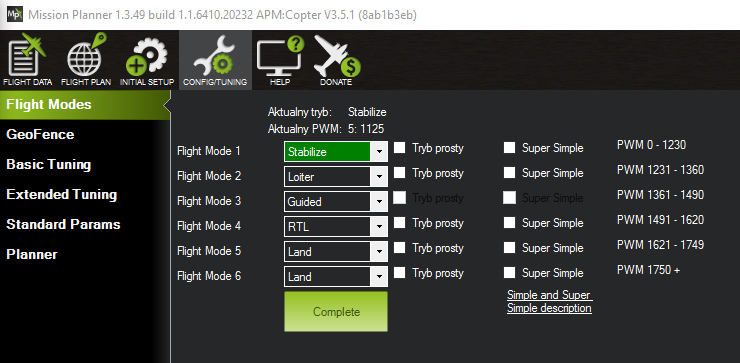
\includegraphics[width=14cm]{B_flight_modes.png}
	\caption{Tryby lotu w oknie konfiguracyjnym aplikacji MISSION Planner}
	\label{fig:flight_modes}
\end{figure}

Opis konfiguracji kanału 5 przedstawiony jest w podrozdziale poświęconym aparaturze radiowej.
\subsection{Protokół MAVLink}
\label{subsec:MAVLink}
Oprogramowanie ArduPilot obsługuje komunikację z urządzeniami pełniącymi rolę stacji naziemnych. Może to być komputer, tablet, ale również obecna na platformie UAV inna jednostka. Niezależnie od wyboru, komunikacja z autopilotem bazuje na wykorzystaniu jednego z jego portów szeregowych \cite{PixhawkSerial}.

Warstwą transportową takiej komunikacji jest protokół MAVLink, opracowany w 2009 roku na potrzeby małych pojazdów bezzałogowych. 
Dość duży podzbiór jego wiadomości i komend jest wspierany przez oprogramowanie ArduCopter (pełna lista jest dostępna pod adresem: \cite{ArduCopterCmds}, dość poręczna jest również strona \cite{MAVLinkMSG}). 
Ramka protokołu ma zmienną długość i jest opisana w tabeli \ref{tab:MAVlinkframe}.

\newcolumntype{P}[1]{>{\centering\arraybackslash}p{#1}}
\begin{table}[h]
	\centering
	\caption{Ramka protokołu MAVLink}
	
	\begin{tabular}{|P{1.5cm} |P{4cm}| p{9cm}|}
		
		\hline
		\rowcolor{lightgray} Bajt \# & Oznaczenie & Uwagi \\ 
		0	& Początek ramki &	Zawsze o wartości 254 \\ \hline
		1	& Długość danych & Wartość \textit{n} (w bajtach )	\\ \hline		
		2	& Sekwencja pakietu &	Wartość inkrementowana z każdą kolejną transmisją\\ \hline
		3	& ID systemu &	Dla komputera pokładowego (SoC) równa 255 \\ \hline
		4	& ID komponentu &	Dla komputera pokładowego (SoC) równa 190 \\ \hline
		5	& ID wiadomości &	\\ \hline
		6:n+6-1	& Dane & Struktura zależna od rodzaju wiadomości	\\ \hline
		n+6:n+7	& CRC &	Suma kontrolna całego pakietu bez bajtu \#0\\ \hline
	\end{tabular}
	\label{tab:MAVlinkframe}
\end{table}

%TODO std. przyjmuje się, że podpisa tabeli powinien być nad. Tu przeniosłem, w pozostałych proszę sprawdzić. %ODP OK

Protokół został zaprojektowany w postaci plików nagłówkowych -- taka forma umożliwia łatwe wykorzystanie w aplikacji tworzonej w języku C/C++.
\subsubsection{Implementacja komend MAVLink}
\label{commands}
Dokumentacja protokołu MAVLink jest dość obszerna, jednak doprowadzenie do pełnego zrozumienia działania poszczególnych komend i ich wpływu na zachowanie drona wymaga podjęcia testów praktycznych.
Każda z komend autopilota ma swój własny plik nagłówkowy, którego najważniejszą częścią jest definicja struktury z danymi, funkcji pakującej (do wysłania wiadomości) oraz dekodującej (do odebrania wiadomości). Mają one dość generyczne nazwy, przykładowo dla wiadomości HEARTBEAT są to odpowiednio:
\begin{itemize}
	\item \textit{mavlink\_heartbeat\_t}
	\item \textit{mavlink\_msg\_heartbeat\_pack(...)}
	\item \textit{mavlink\_msg\_heartbeat\_decode(...)}
\end{itemize}
Używanie tych funkcji ma dodatkową zaletę - uwzględniają liczenie sumy kontrolnej oraz sekwencji pakietu, a więc elementów, których błędne wartości powodowałaby nieprawidłowości w transmisji.
Do komunikacji pomiędzy urządzeniami wykorzystywany jest port szeregowy, zatem najmniejszą jednostką wymiany informacji jest bajt. Dla procesu odbierania wiadomości należy ten zestaw bajtów odpowiednio zinterpretować -- do formowania ich w ramki służy funkcja \textit{mavlink\_frame\_char(...)}, która powinna być wywoływana w trakcie odebrania każdego bajtu danych. Zwracany przez nią status określa, czy ramka jest już gotowa do dalszej analizy. Pełna wiadomość zostanie przepisana do struktury typu \textit{mavlink\_message\_t}. Jedno z z pól gotowej struktury, \textit{msgid}, określa typ wiadomości. Pozwala to zdefiniować użycie odpowiedniej funkcji dekodującej w zależności od ID - gotowe informacje będą się znajdować w odpowiedniej strukturze danych.\newline
Przykładowo, ID o numerze 253 oznacza wiadomość typu STATUSTEXT (informacja z autopilota w formacie tekstowym). W celu jej zdekodowania należy wywołać funkcję 
\textit{mavlink\_msg\_statustext\_decode(...)}, która zwróci strukturę \textit{mavlink\_statustext\_t} ze znakami gotowymi do wyświetlenia lub dalszej analizy.

Wysyłanie komend jest o wiele prostsze, wymagane jest bowiem spakowanie informacji w tablicę bajtów i wysyłanie ich w odpowiedniej kolejności.

Najbardziej skomplikowaną w użyciu jest komenda ruchu, SET\_POSITION\_TARGET\_LOCAL\_NED. Funkcja, która jest odpowiedzialna za konwersję jej w tablicę bajtów nosi nazwę \textit{mavlink\_msg\_set\_position\_target\_local\_ned\_pack}. Używa ona następujących parametrów
\begin{itemize}
	\item \textit{x, y, z} -- przesunięcie w odpowiednim kierunku, w metrach
	\item \textit{vx, vy, vz} -- prędkość w odpowiednim kierunku, w $m/s$
	\item \textit{afx, afy, afz} -- przyśpieszenie w odpowiednim kierunku, w $m/s^2$ lub $N$
	\item \textit{yaw} -- obrót wokół pionowej osi, w radianach
	\item \textit{yaw\_rate} -- prędkość kątowa obrotu, w rad/s
	\item \textit{type\_mask} -- maska bitowa określająca wartości, które mają być zignorowane (wartość 1) przez autopilot. Mapowanie bitów 1: x, bit 2: y, bit 3: z, bit 4: vx, bit 5: vy, bit 6: vz, bit 7: ax, bit 8: ay, bit 9: az, bit 11: yaw, bit 12: yaw\_rate. Bit 10 jest używany do określenia jednostki przyśpieszenia
	\item \textit{coordinate\_frame} -- zdefiniowanie układu współrzędnych, w odniesieniu do którego odbywać się będzie ruch
\end{itemize}
Warto zaznaczyć, że do wykonania ruchu potrzebne jest odblokowanie wszystkich bitów związanych z przemieszczeniem LUB prędkością, kombinacja obu sposobów ruchu nie jest wspierana przez oprogramowanie ArduPilot. Parametry związane z przyśpieszeniem oraz obrotem w osi pionowej również nie są wspierane.
Do przechowywania wartości wygodnie jest używać struktury \textit{mavlink\_set\_position\_target\_local\_ned\_t}.

\section{Konfiguracja aparatury radiowej}

Aparatura radiowa FrSky Taranis X9D Plus pozwala przesyłać informacje zgrupowane w 16 kanałów. Do manualnej kontroli drona wymagane są jedynie 4 z nich, przyporządkowane dwóm głównym drążkom aparatury. Najważniejszym sygnałem jest Throttle, który odpowiada za ogólny poziom mocy wszystkich silników drona. Kolejnymi sygnałami są Roll, Pitch oraz Yaw, które są przyporządkowane osiom obrotu platformy \ref{fig:flight_modes}.

\begin{figure}[ht]
	\centering
	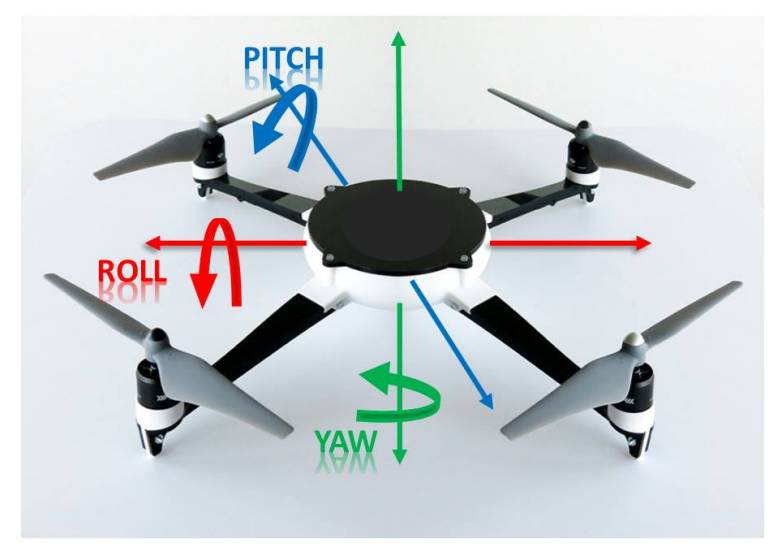
\includegraphics[width=12cm]{B_rotational_axes.png}
	\caption{Osi obrotu drona \cite{Bouhali2017}}
	\label{fig:flight_modes}
\end{figure}

Kanał 5 jest używany przez autopilota do zmiany trybu lotu. Funkcja ta obsługuje wybór spośród maksymalnie 6 trybów, którym przyporządkowano zakresy szerokości pulsu PWM przedstawione w oknie konfiguracyjnym \ref{fig:flight_modes}. Elementem aparatury radiowej przypisanym do kanału musiał zostać zestaw kilku przełączników - zastosowanie potencjometrów nie byłoby ergonomicznym rozwiązaniem. Wybrano dwa przełączniki 3-pozycyjne oznaczone jako SA oraz SB, które mikser aparatury dodaje do siebie - przedstawia to rysunek \ref{fig:mixer}. Zastosowane wagi: $-30$ dopasowano, by położenie dolne obu przełączników odpowiadało trybowi 1, a zmiana stanu któregokolwiek z nich skutkowała przejściem do innego zakresu szerokości pulsu PWM. Ostatecznie zestaw obu przełączników daje możliwość wyboru spośród 5 trybów lotu.
\begin{figure}[ht]
	\centering
	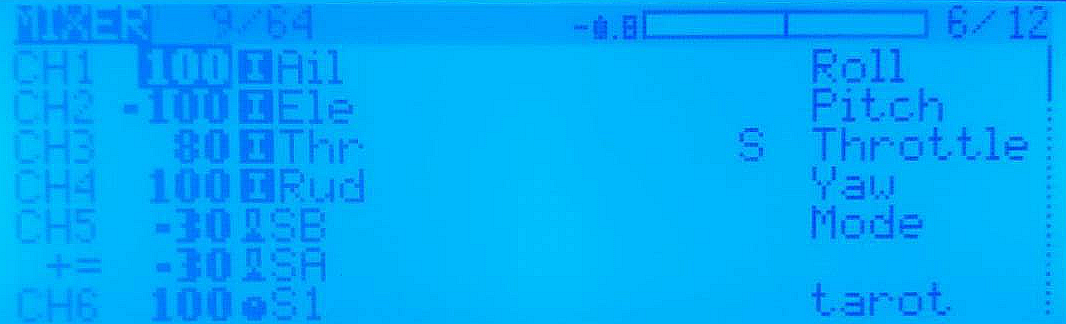
\includegraphics[width=10cm]{B_mixer.png}
	\caption{Mikser sygnałów w aparaturze radiowej}
	\label{fig:mixer}
\end{figure}

Kanał 6 jest przypisany do potencjometru S1 i został skonfigurowany jako sygnał ciągły sterujący wartością zadaną nachylenia kamery. W trakcie lotu  mechanizmy gimbala utrzymują tę wartość pomimo możliwych wychyleń platformy. Orientacja kamery z minimalną wartością nachylenia pozwala rejestrować obraz bezpośrednio przed dronem, z kolei maksymalna wartość nachylenia kieruje obiektyw ku ziemi.\newline
Ważne: ze względu na podłączony do kamery przewód HDMI regulacja nachylenia nie działa poprawnie -- w projekcie zasilanie silnika odpowiedzialnego za nachylenie kamery nie jest podłączone.
%może jakaś kalibracja żyroskopów gimbala jest w stanie pomóc, na pewno przydałby się bardziej giętki kabel

Kanał 7 przypisano do 3-pozycyjnego przełącznika SC. Sygnał PWM z informacją z tego kanału jest wysyłany przez autopilot do układu rekonfigurowalnego i służy do zdalnego rozpoczęcia misji śledzenia.


\section{Instrukcja powtórzenia eksperymentu śledzenia}

\begin{itemize}
	\item Upewnić się, że wszystkie przewody zostały poprawnie podłączone do płyty PYNQ (zasilanie 5V, sygnały z autopilota), a sama płyta jest dobrze unieruchomiona na platformie
	\item Podłączyć pakiet LiPo
	\item Włączyć zasilanie płyty PYNQ
	\begin{itemize}
		\item jeśli układ Zynq nie jest konfigurowany z karty SD, należy skonfigurować go poprzez port USB-JTAG
	\end{itemize}	
	\item Włączyć kamerę i upewnić się, że jest w trybie rejestracji wideo
	\item Podłączyć autopilot do komputera (kabel USB) i w aplikacji MISSION Planner sprawdzić podstawowe informacje -- obecność sygnału GPS i innych czujników, zwracane błędy. Zamknąć połączenie i odłączyć kabel
	\item Upewnić się, że nie ma przewodów lub elementów mogących stanowić zagrożenie podczas pracy silników
	\item Włączyć aparaturę radiową i za pomocą przełączników SA oraz SB wybrać tryb GUIDED
	\item Ustawić przełącznik SC w pozycji górnej -- wysłać sygnał rozpoczynający misję 
	\item Oczekiwać na osiągnięcie stałej wysokości przez drona przy zachowaniu pozycji stojącej i odległości kilku metrów od platformy
	\item Po ruchu drona wskazującym na rozpoczęcie śledzenia, można zmienić swoje położenie i obserwować działanie systemu 
	\item Wyłączyć misję ustawieniem przełącznika SC w pozycji środkowej lub dolnej -- rozpocznie się lądowanie 
\end{itemize}